\chapter{Application Design}\label{chapter::decentralizedapps}

\section{Introduction}
	An Application software or \textit{app} is a computer program designed to perform a specific set of tasks or actions for the end user. There are countless number of applications in use today and the majority of them are web applications following a centralized client-server model\cite{raval2016decentralized}.
	
	\begin{figure}[h]
		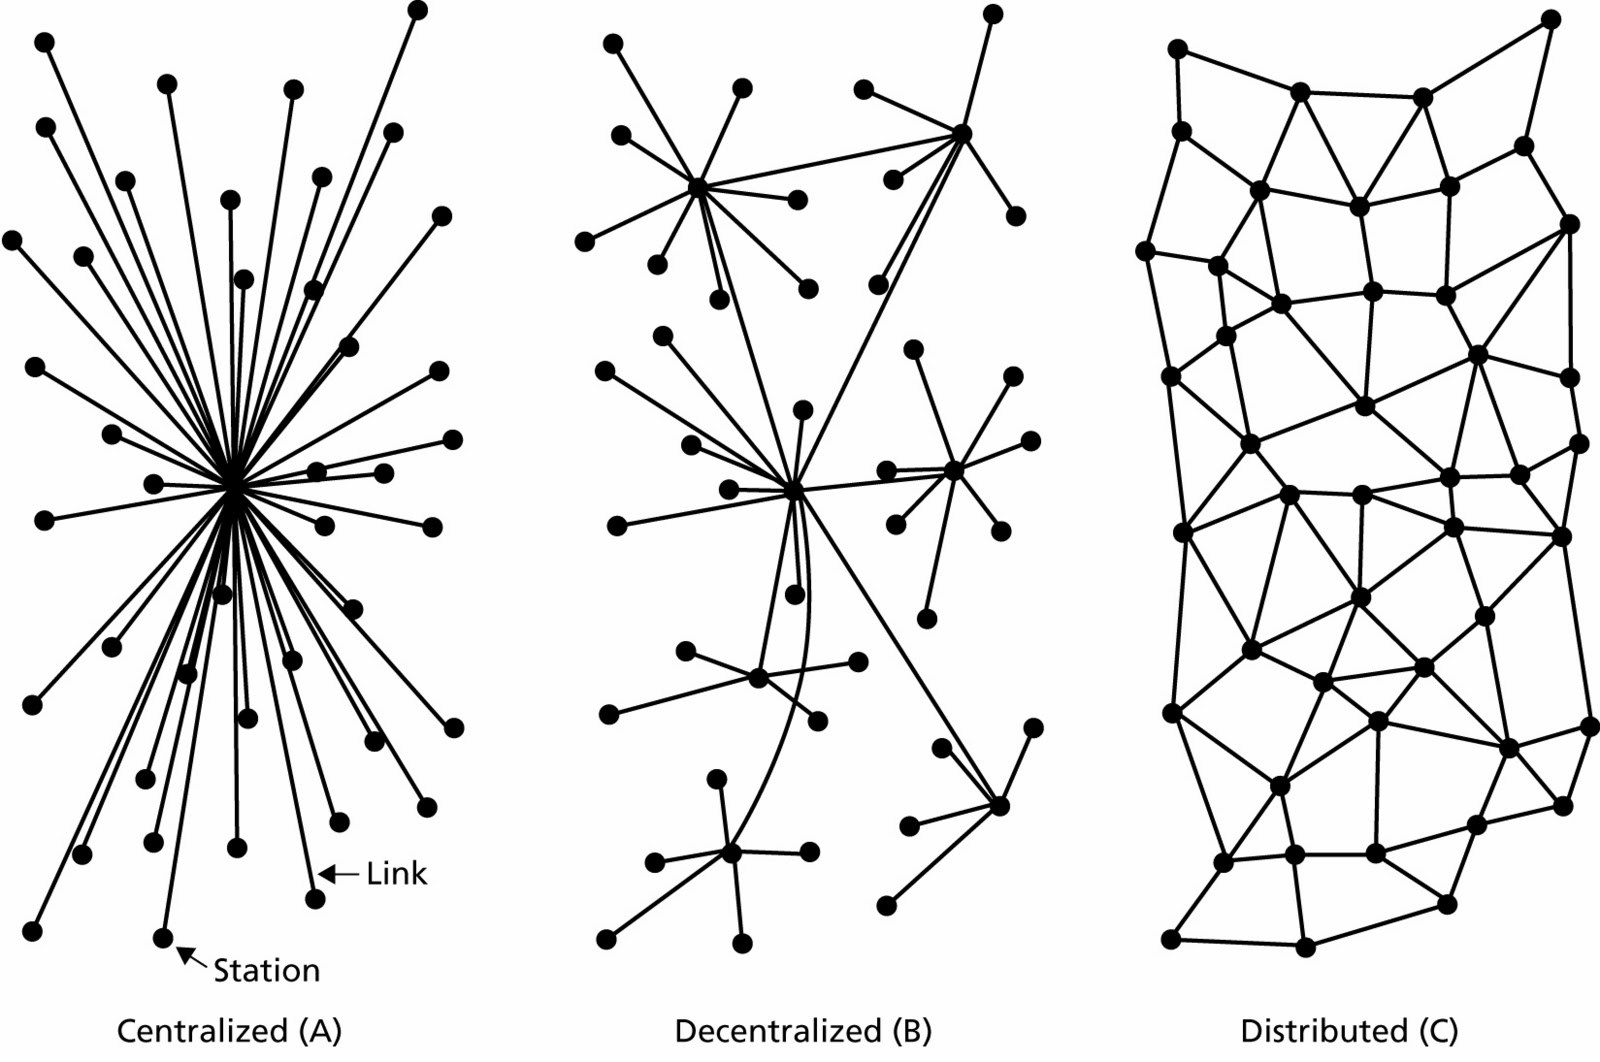
\includegraphics[width=\linewidth]{figures/network-models}
		\caption{\label{fig:applications} The three way of modeling web applications}
	\end{figure}
	
	Figure~\ref{fig:applications} shows a visual representation of three different ways of modeling web applications\cite{baran1964distributed}. Here, \textit{Centralized} and \textit{Decentralized} refers to level of control, while \textit{Distributed} refers to differences of location. Both centralized and decentralized systems can be distributed as well.
	
	\subsection{Centralized}
	It's currently the widespread way of building software applications. In this model a central server control the flow of information and governs the operation of individual units. Since the control is centralized, these types of systems suffer from single point of failure risk.
	
	\subsection{Distributed}
	In a Distributed model, the control still resides with a central server, however, the computation is spread across multiple nodes or servers.
	
	\subsection{Decentralized}
	In a Decentralized model, there is no central point of control as it's spread across all the servers running the application. Applications built using this model don't have a single point of failure and are inherently fault tolerant.

\section{Enabling Technologies}
	The document \textit{Information Management: A Proposal\cite{berners1989information}} written by \textit{Sir Tim Berners-Lee\footnote{\url{https://www.w3.org/People/Berners-Lee/}}} conceived the ideas for what would become the WorldWideWeb. It's main goal was to enable information exchange between computers in an accessible way at CERN\footnote{\url{https://home.cern/}}.
	
	HTML\footnote{\url{https://developer.mozilla.org/en-US/docs/Web/HTML}}, URI\footnote{\url{https://tools.ietf.org/html/rfc3986}} and HTTP\footnote{\url{https://tools.ietf.org/html/rfc2616}} were the fundamental technologies that defined the foundation of the Web. HTTP connected every computer on the planet with a common protocol. The HTTP protocol guidelines defined a set of trusted servers that translated a web address into a server address. Furthermore, HTTPS\footnote{\url{https://tools.ietf.org/html/rfc2818}} added another layer of trusted servers and certificate authorities. People would host personal servers for others to connect to, and everyone owned their data\cite{raval2016decentralized}. As the Web evolved, applications servers\footnote{\url{https://en.wikipedia.org/wiki/Application_server}} became the common way of interactive with the Web and the centralized model of data ownership as we know it today was born\cite{raval2016decentralized}. It was conceptually and programmatically easier to maintain an application server and profit from user's data that utilize it.
	
	Blockchain is the primary technology that enables the creation of applications with a decentralized model of data ownership. It puts the users of an application in control of their data thereby enabling a more open Web, as it was originally intended\footnote{\url{https://webfoundation.org/about/vision/history-of-the-web/}}.
	
	The blockchain helped solve the Byzantine Generals Problem\cite{lamport1982byzantine}. This problem describes a situation where all participating nodes in a distributed network must agree upon every message that is being transmitted between nodes, but where some of the nodes are corrupt and disseminating false information or are unreliable. This agreement is called as \textbf{consensus}. With Bitcoin\cite{nakamoto2008bitcoin}, decentralized consensus became possible. Agreement is achieved in the Bitcoin network by way of \textit{proof-of-work\footnote{\url{https://en.bitcoin.it/wiki/Proof_of_work}}} consensus mechanism which is resistant to Sybil Attack\cite{douceur2002sybil}. Proof-of work is both computationally and energy expensive; other consensus mechanism such as \textit{proof-of-stake\footnote{\url{https://en.bitcoin.it/wiki/Proof_of_Stake}}} relies on stake in the system instead of computational power.
	
	\section{Concepts}
	There are five concepts in a web application that have traditionally been implemented in way that puts control with a centralized entity: data, identity, value, computing and bandwidth\cite{raval2016decentralized}. Each of these require trust in a 3rd party - a trust which can be betrayed. Recent advancements in distributed-system technology can put users in control of these things. Below sections describes each concept in detail and shows how one can build applications in a way such that centralized control is not required.

	\subsection{Data}
	Data is the most important concept in any web application. First, let's look at how traditional web applications interact with data. Whenever, a user logs into an application, the application connects to a remote server and sends the authentication details. These details lets the server know which user is interacting with the application. Once authenticated, the user data is fetched from the remote storage and displayed to the user. All complex computations and data storage occurs on dedicated servers maintained in the cloud.
	
		\subsubsection{1: Storing Data Directly in a Blockchain}
		
		\subsubsection{2: Storing Data in a Distributed Hash Table}
		
		\subsubsection{3: Storing Data in a Cloud in Encrypted Containers}
	
	\subsection{Identity}
	
	\subsection{Value}
	
	\subsection{Computing}
	
	\subsection{Bandwidth}